\section{\K 稳压二极管}
\Par 稳压二极管管如其名,是用来稳压的.稳压二极管工作于反向击穿区,在反向击穿状态下,反向电流在一定范围内变化时,稳压二极管两端的电压变化很小,利用这一特性,可以实现“稳电”作用.

\begin{figure}[htbp]
	\centering
	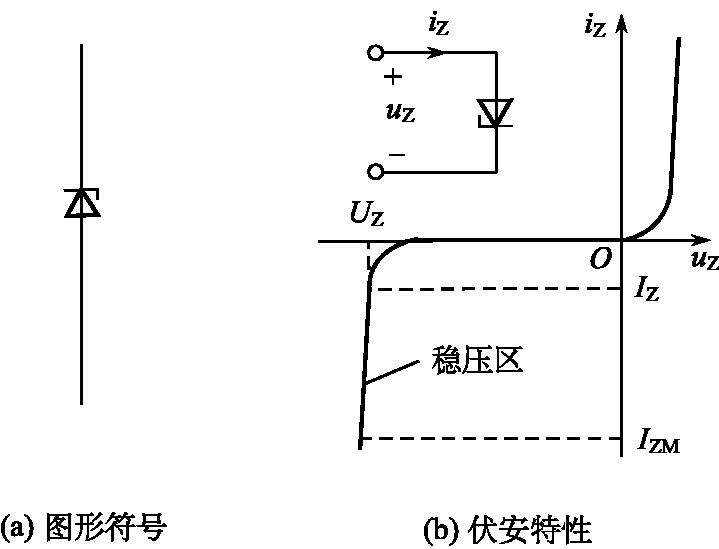
\includegraphics[width=0.35\textwidth]{稳压二极管.jpg}
	\caption{稳压二极管}
	\label{fig:稳压二极管}
\end{figure}

\Par 工作时的稳压二极管电路如图\ref{fig:稳压电路}所示.试分析:当$R_L$变大时,并联结构的总电阻变大,从而它的分压变大,根据图\ref{fig:稳压二极管}中的图(b),我们可以知道,$D_Z$的电压稍一增大,电流就大幅增加,由于电路中的总电流减小,因此$R_L$支路的电流会减小.电阻变大,但是电流变小,因此$R_L$两端电压会维持恒定

\Par 当电源电压$U$变大时,稳压二极管两端的分压也会变大,根据图\ref{fig:稳压二极管}中的图(b),我们可以知道,$D_Z$的电压稍一增大,电流就大幅增加,从而电路的电流也会大幅增加,让$R_I$的电压变大,从而分走$U$变大的电压,让$R_L$两端电压维持恒定.

\begin{figure}[htbp]
	\centering
	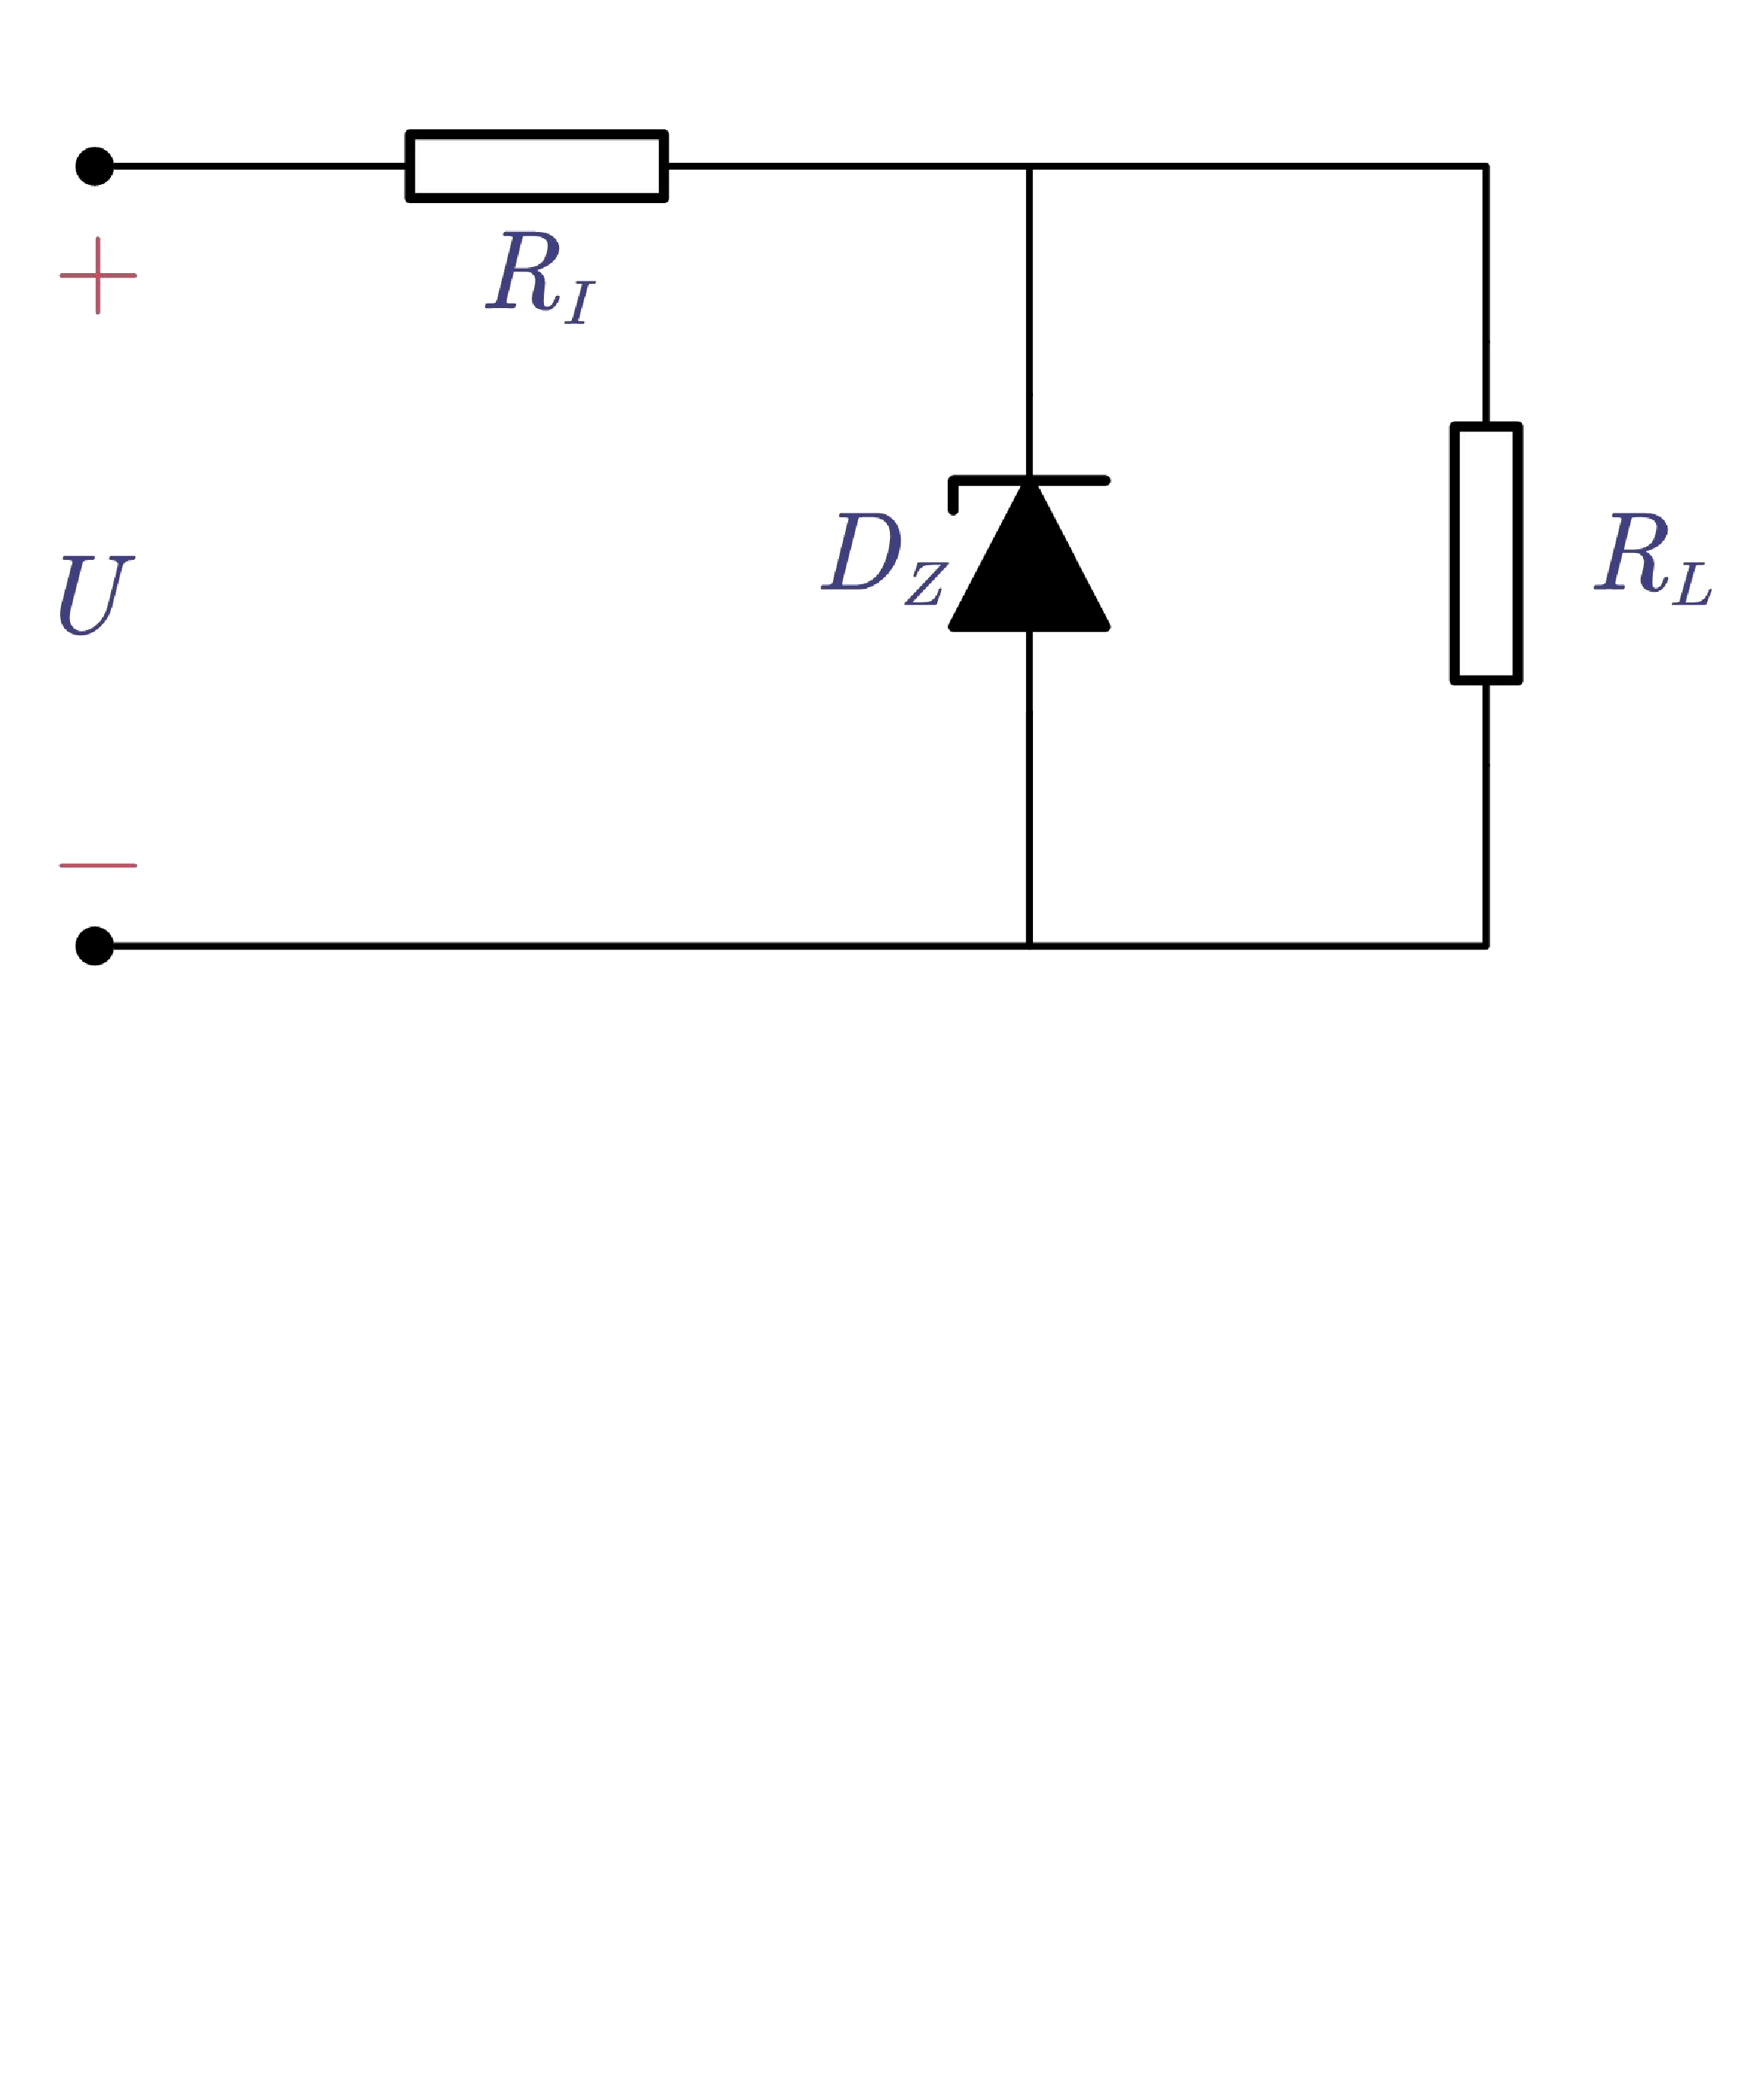
\includegraphics[width=0.45\textwidth]{稳压电路.pdf}
	\caption{稳压电路}
	\label{fig:稳压电路}
\end{figure}

